%%%%%%%%%%%%%%%%%%%%%%%%%%%%%%%%%%%%%%%%%%%%%%%%%%%%%%%%%%%%%%%%%%%%%%%%%%%%%%%%
\section{Why quantum computing?}
%%%%%%%%%%%%%%%%%%%%%%%%%%%%%%%%%%%%%%%%%%%%%%%%%%%%%%%%%%%%%%%%%%%%%%%%%%%%%%%%
\begingroup
\nologo
%%%%%%%%%%%%%%%%%%%%%%%%%%%%%%%%%%%%%%%%%%%%%%%%%%%%%%%%%%%%%%%%%%%%%%%%%%%%%%%%
\subsection{Moore's law}
\begin{frame}{}
    \centering
    \includegraphics[width=0.75\textwidth]{pics/introduction/Transistor-Count-over-time-to-2018.png}
\end{frame}
%%%%%%%%%%%%%%%%%%%%%%%%%%%%%%%%%%%%%%%%%%%%%%%%%%%%%%%%%%%%%%%%%%%%%%%%%%%%%%%%
\begin{frame}{}
    \centering
    \Large Moore's Law\\
    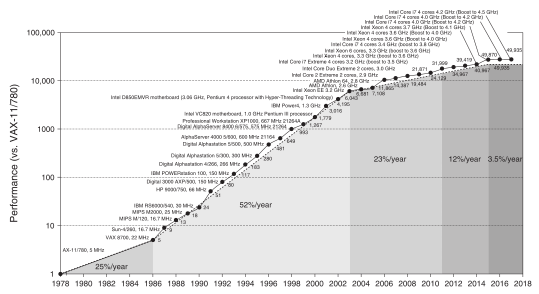
\includegraphics[width=0.9\textwidth]{pics/introduction/computer_arch.pdf}
    \source{Hennessy, John L., and David A. Patterson. Computer
    architecture: a quantitative approach. Elsevier, 2011. 6th edition.}
\end{frame}
\endgroup
%%%%%%%%%%%%%%%%%%%%%%%%%%%%%%%%%%%%%%%%%%%%%%%%%%%%%%%%%%%%%%%%%%%%%%%%%%%%%%%%
\begingroup
\nologo
\begin{frame}{}
    \centering
    \includegraphics[width=0.7\textwidth]{pics/introduction/50-years-processor-trend.pdf}
    \source{\url{https://github.com/karlrupp/microprocessor-trend-data}}
\end{frame}
%%%%%%%%%%%%%%%%%%%%%%%%%%%%%%%%%%%%%%%%%%%%%%%%%%%%%%%%%%%%%%%%%%%%%%%%%%%%%%%%
\subsection{Amdhal's law}
\begin{frame}{}
    \centering
    \includegraphics[width=0.75\textwidth]{pics/introduction/AmdahlsLaw.pdf}
\end{frame}
\endgroup
%%%%%%%%%%%%%%%%%%%%%%%%%%%%%%%%%%%%%%%%%%%%%%%%%%%%%%%%%%%%%%%%%%%%%%%%%%%%%%%%
\subsection{Patents in quantum computing and quantum machine learning}
\begin{frame}[allowframebreaks]{}
    \centering
    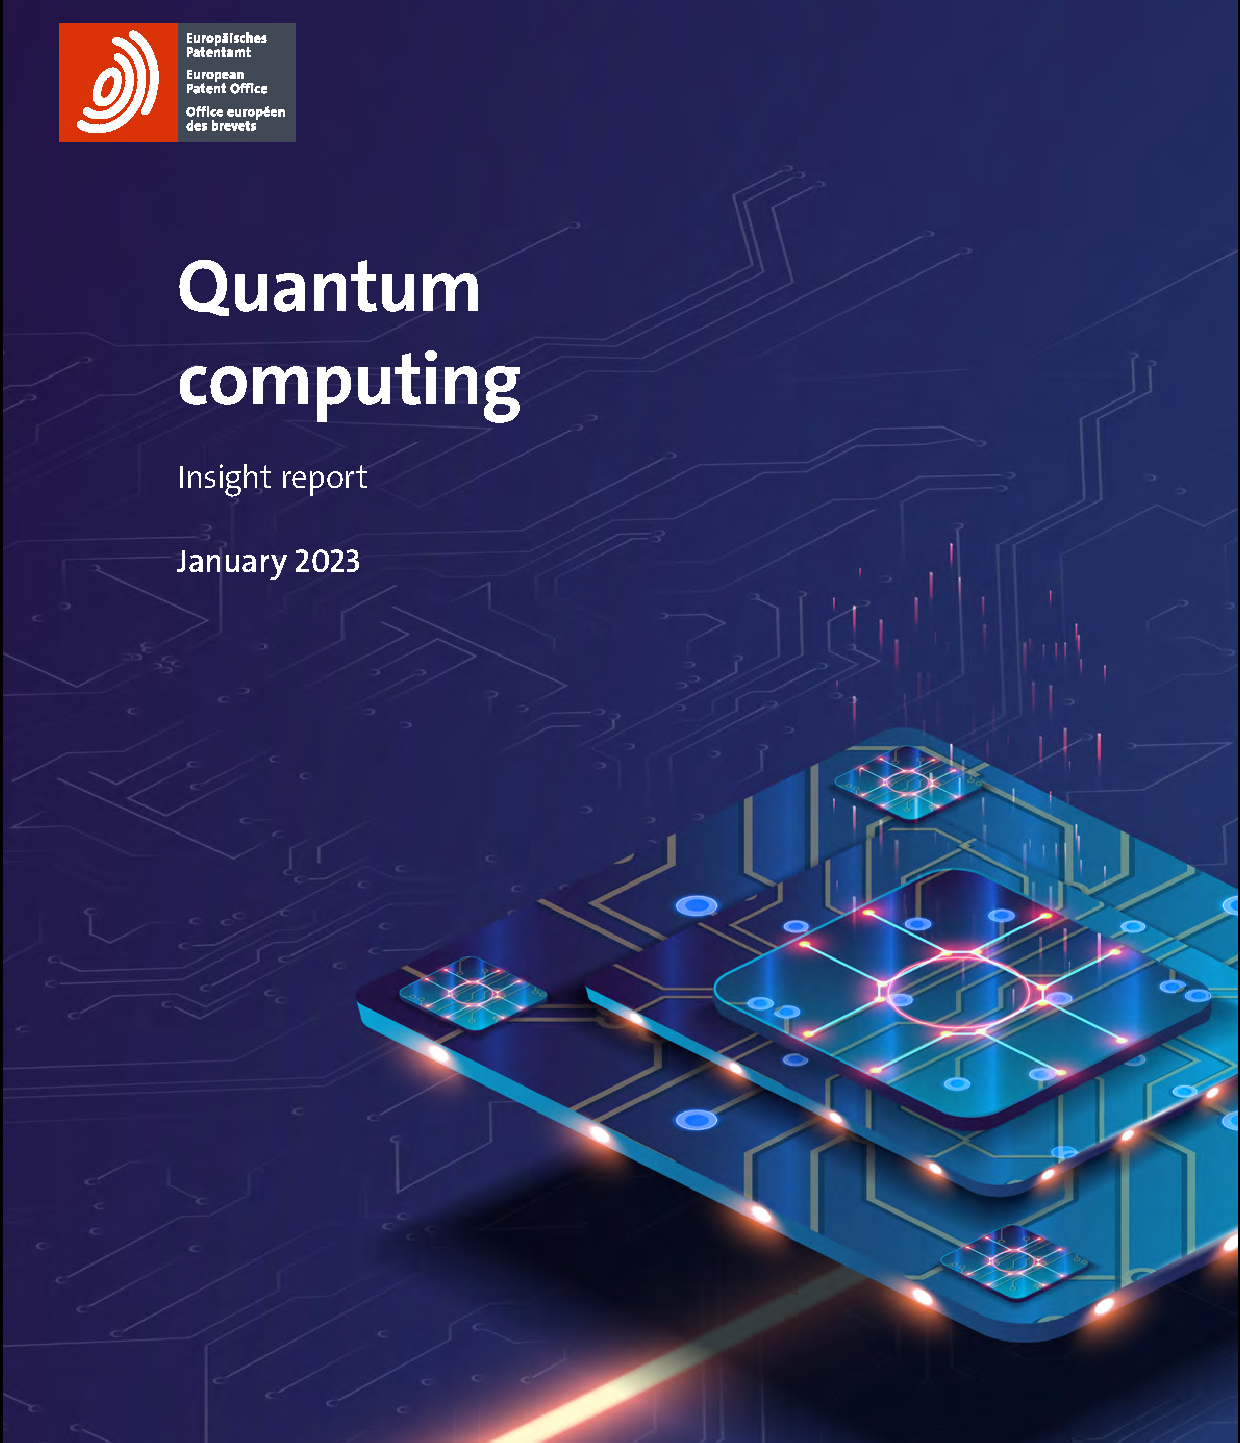
\includegraphics[width=0.5\textwidth, page=1]{pics/introduction/patents.pdf}\\
    \includegraphics[width=0.75\textwidth, page=2]{pics/introduction/patents.pdf}\\
    \includegraphics[width=0.75\textwidth, page=3]{pics/introduction/patents.pdf}\\
\end{frame}
%%%%%%%%%%%%%%%%%%%%%%%%%%%%%%%%%%%%%%%%%%%%%%%%%%%%%%%%%%%%%%%%%%%%%%%%%%%%%%%%
\section{Introduction to the quantum world}
%%%%%%%%%%%%%%%%%%%%%%%%%%%%%%%%%%%%%%%%%%%%%%%%%%%%%%%%%%%%%%%%%%%%%%%%%%%%%%%%
\subsection{Interference}
\begin{frame}{Interference}
    \includegraphics[width=0.98\textwidth]{pics/ds_exp.jpg}\\
    Classical: $I_{1+2}=I_1 + I_2$\\
    Quantum: $I_{12}=I_1 + I_2 + 2\sqrt{I_1 I_2} \cos(\theta_1 - \theta_2)$\\
    $I_{12}=|\alpha_1+\alpha_2|^2, \alpha_i \in \mathbb{C}, \alpha_i=|\alpha_i|e^{\mathrm{i}\theta_i}.$
\end{frame}
%%%%%%%%%%%%%%%%%%%%%%%%%%%%%%%%%%%%%%%%%%%%%%%%%%%%%%%%%%%%%%%%%%%%%%%%%%%%%%%%
\begin{frame}{Interference}
    \centering
    \includegraphics[width=0.8\textwidth]{pics/ds_pattern.jpg}
\end{frame}
%%%%%%%%%%%%%%%%%%%%%%%%%%%%%%%%%%%%%%%%%%%%%%%%%%%%%%%%%%%%%%%%%%%%%%%%%%%%%%%%
\subsection{Mach-Zender interferometer}
%%%%%%%%%%%%%%%%%%%%%%%%%%%%%%%%%%%%%%%%%%%%%%%%%%%%%%%%%%%%%%%%%%%%%%%%%%%%%%%%
\begin{frame}[allowframebreaks]{Mach-Zender interferometer}
    \newlength{\wdth}
    \centering
    \setlength{\wdth}{0.5\textwidth}
    \includegraphics[width=\wdth]{pics/bombs/Mach-Zehnder_interferometer_k0}\\
    \includegraphics[width=\wdth]{pics/bombs/Mach-Zehnder_interferometer_k1}\\
    \includegraphics[width=\wdth]{pics/bombs/Mach-Zehnder_interferometer_pomiar_1}\\
    \includegraphics[width=\wdth]{pics/bombs/Mach-Zehnder_interferometer_pomiar_2}\\
    \source{Wikimedia, \copyright{} Ansgar Hellwig 2005, public domain.}
\end{frame}
%%%%%%%%%%%%%%%%%%%%%%%%%%%%%%%%%%%%%%%%%%%%%%%%%%%%%%%%%%%%%%%%%%%%%%%%%%%%%%%%
\subsection{Elitzur-Vaidman bomb testing problem}
\begin{frame}[allowframebreaks]{Elitzur-Vaidman bomb testing problem}
    \centering
    \centering
    \setlength{\wdth}{0.6\textwidth}
    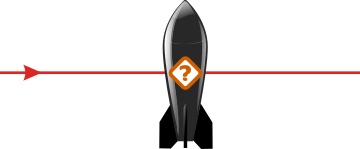
\includegraphics[width=\wdth]{pics/bombs/Mach-Zehnder_interferometer_bomby}\\
    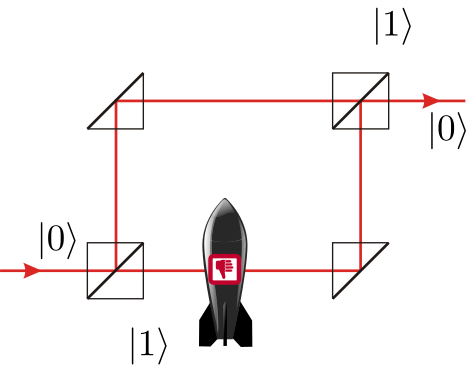
\includegraphics[width=\wdth]{pics/bombs/Mach-Zehnder_interferometer_bomby_zla}\\
    \begin{overpic}[width=\wdth]{pics/bombs/Mach-Zehnder_interferometer_bomby_dobra}
        \put(-50,71){
        \begin{tabular}{c|c|c|c}
            p &explosion & result & conclusion \\ \hline
            1/2 & yes & --- & was good\\
            1/4 & no & $0$ & don't know\\
            1/4 & no & $1$ & good
        \end{tabular}
        }
    \end{overpic}\\
\end{frame}

%%%%%%%%%%%%%%%%%%%%%%%%%%%%%%%%%%%%%%%%%%%%%%%%%%%%%%%%%%%%%%%%%%%%%%%%%%%%%%%%
\section{Bibliography}
\begin{frame}[noframenumbering,plain,allowframebreaks]{Bibliography}
    \nocite{*}
    \printbibliography
\end{frame}
%%%%%%%%%%%%%%%%%%%%%%%%%%%%%%%%%%%%%%%%%%%%%%%%%%%%%%%%%%%%%%%%%%%%%%%%%%%%%%%%
\section{Building blocks of quantum world}
\subsection{Classical and quantum computing}
\begin{frame}{Quantum computers are not self-sufficient}
    \begin{figure}
        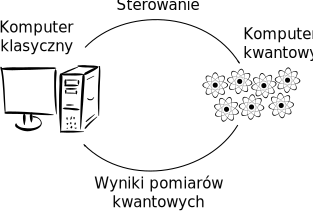
\includegraphics[scale=1]{pics/sterowaniepomiar}
    \end{figure}
\end{frame}
%%%%%%%%%%%%%%%%%%%%%%%%%%%%%%%%%%%%%%%%%%%%%%%%%%%%%%%%%%%%%%%%%%%%%%%%%%%%%%%%
\begin{frame}{Scheme of a quantum device}
    \begin{figure}
        \includegraphics[scale=0.7]{pics/experiment}
    \end{figure}
\end{frame}
%%%%%%%%%%%%%%%%%%%%%%%%%%%%%%%%%%%%%%%%%%%%%%%%%%%%%%%%%%%%%%%%%%%%%%%%%%%%%%%%
\subsection{Quantum states}
%%%%%%%%%%%%%%%%%%%%%%%%%%%%%%%%%%%%%%%%%%%%%%%%%%%%%%%%%%%%%%%%%%%%%%%%%%%%%%%%
\begin{frame}{Bits and qubits}
    \begin{columns}
        \begin{column}[t]{0.5\textwidth}
            \begin{center}
                \huge
                Bit\\
                $0$ or $1$
            \end{center}
        \end{column}
        % \vrule{}
        \begin{column}[t]{0.5\textwidth}
            \begin{center}
                \huge
                Qubit\\
                $\alpha\ket{0}+\beta\ket{1}$
            \end{center}
        \end{column}
    \end{columns}
\end{frame}
%%%%%%%%%%%%%%%%%%%%%%%%%%%%%%%%%%%%%%%%%%%%%%%%%%%%%%%%%%%%%%%%%%%%%%%%%%%%%%%%
\begin{frame}{Mathematical properties of qubits}
    \begin{center}
        \Large
        $\ket{\psi} = \alpha\ket{0}+\beta\ket{1} =
        \begin{bmatrix}
            \alpha \\
            \beta
        \end{bmatrix}$\\[1cm]
        $|\alpha|^2 + |\beta|^2=1$\\[1cm]
        $e^{i\phi}\ket{\psi}\equiv \ket{\psi}$
        \\[1cm]
    \end{center}
\end{frame}
%%%%%%%%%%%%%%%%%%%%%%%%%%%%%%%%%%%%%%%%%%%%%%%%%%%%%%%%%%%%%%%%%%%%%%%%%%%%%%%%
\begin{frame}{Dirac bra-ket notation}
    Let 
    \begin{equation*}
        \ket{\psi} = %\alpha\ket{0}+\beta\ket{1} =
        \begin{bmatrix}
            \alpha \\
            \beta
        \end{bmatrix},
        \quad 
        \ket{\phi} = %\alpha\ket{0}+\beta\ket{1} =
        \begin{bmatrix}
            \gamma \\
            \delta
        \end{bmatrix},
        \quad 
        \bra{\psi} = \ket{\psi}^\dagger = \begin{bmatrix}
            \overline{\alpha}, \overline{\beta} 
        \end{bmatrix}.
    \end{equation*}
    
    Properties:
    \begin{itemize}
        \item inner (scalar) product
        \begin{equation*}
            \braket{\psi}{\phi}
            = 
            \begin{bmatrix}
                \overline{\alpha}, \overline{\beta} 
            \end{bmatrix}
            \begin{bmatrix}
                \gamma \\
                \delta
            \end{bmatrix}
            =\overline{\alpha} \gamma +  \overline{\beta} \delta,
        \end{equation*}
        
        \item length
        \begin{equation*}
            \sqrt{\braket{\psi}{\psi}}
            %\begin{bmatrix}
                %\overline{\alpha}, \overline{\beta} 
                %\end{bmatrix}
                %\begin{bmatrix}
                    %\alpha \\
                    %\beta
                    %\end{bmatrix}
                    = \sqrt{|\alpha|^2 +  |\beta|^2} = 1,
                \end{equation*}
                
                \item outer product
                \begin{equation*}
                    \ketbra{\psi}{\phi} = 
                    \begin{bmatrix}
                        \alpha \\
                        \beta
                    \end{bmatrix}
                    \begin{bmatrix}
                        \overline{\gamma} & \overline{\delta}
                    \end{bmatrix}
                    =
                    \begin{bmatrix}
                        \alpha \overline{\gamma} &  \alpha \overline{\delta}\\
                        \beta \overline{\gamma} &   \beta \overline{\delta}
                    \end{bmatrix}.
                \end{equation*}
            \end{itemize}
        \end{frame}
        %%%%%%%%%%%%%%%%%%%%%%%%%%%%%%%%%%%%%%%%%%%%%%%%%%%%%%%%%%%%%%%%%%%%%%%%%%%%%%%%
        \begin{frame}{Representation of qubits}
            \begin{figure}
                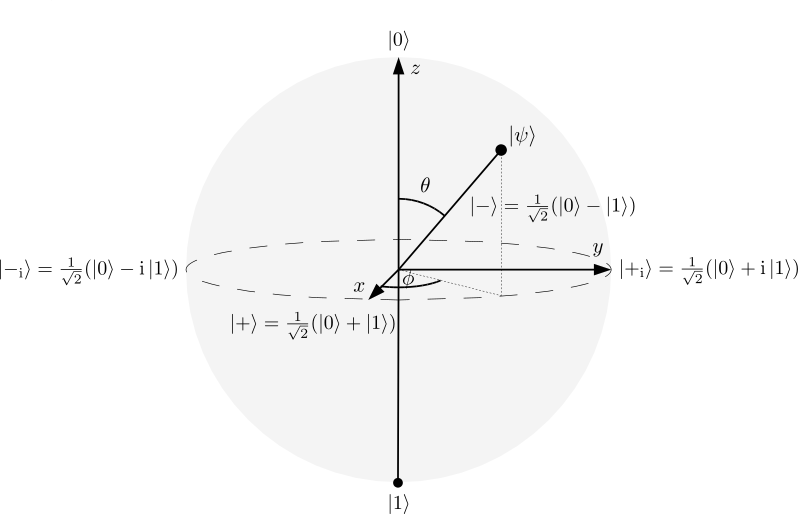
\includegraphics[scale=0.5]{pics/bloch}
            \end{figure}
        \end{frame}
        %%%%%%%%%%%%%%%%%%%%%%%%%%%%%%%%%%%%%%%%%%%%%%%%%%%%%%%%%%%%%%%%%%%%%%%%%%%%%%%%
        \subsection{Quantum measurements}
        %%%%%%%%%%%%%%%%%%%%%%%%%%%%%%%%%%%%%%%%%%%%%%%%%%%%%%%%%%%%%%%%%%%%%%%%%%%%%%%%
        \begin{frame}{Measurement}
            Quantum measurement is a function $\mu$: 
            \begin{itemize}
                \item from finite set of measurements outcomes $A=\{a_i\}_{i=0}^{n-1}$
                \item to set the of projection operators  $P=\{P_i\}_{i=0}^{n-1}$ (where projections satisfy $P_i^2=P_i$) such that $$	\sum_{i=0}^{n-1} P_i = \mathbb{I}.$$	
            \end{itemize}
        \end{frame}
        
        \begin{frame}{Measurement}
            The \textbf{probability of measuring outcome} $a_i$ given the quantum 
            system in in state $\ket{\psi}$ is
            $$
            p(a_i)=\bra{\psi}P_i\ket{\psi}.
            $$
            The state of the quantum system \textbf{after the measurement} outcome 
            $a_i$ was obtained becomes
            $$
            \ket{\psi}_{a_i} = \frac{P_i\ket{\psi}}{\sqrt{\bra{\psi}P_i\ket{\psi}}}.
            $$
        \end{frame}
        %%%%%%%%%%%%%%%%%%%%%%%%%%%%%%%%%%%%%%%%%%%%%%%%%%%%%%%%%%%%%%%%%%%%%%%%%%%%%%%%
        \begin{frame}{Example~$1$ --- part~I}
            \begin{block}{We will measure the state}
                %\vspace{-0.2cm}
                $$\ket\psi = \sqrt{0.7} \ket{0} + \sqrt{0.3} \mathrm{i} \ket{1} $$
            \end{block}
            \begin{block}{by a measurement}
                %\vspace{-0.4cm}
                \begin{equation*}
                    A = \{0,1\}, \quad  P = \left\{P_0  = 
                    \begin{bmatrix}
                        1 & 0\\
                        0 & 0
                    \end{bmatrix}, \ 
                    P_1 = 
                    \begin{bmatrix}
                        0 & 0\\
                        0 & 1
                    \end{bmatrix}\right\}.
                \end{equation*}
            \end{block}
            
            \begin{block}{Probabilities of obtaining outcomes $0$ and $1$}
                \vspace{-0.4cm}
                \begin{equation*}
                    \begin{split}
                        p(0) &= \bra{\psi} P_0 \ket{\psi} = 
                        \begin{bmatrix}
                            \sqrt{0.7} & -\sqrt{0.3} \mathrm{i}
                        \end{bmatrix}
                        \begin{bmatrix}
                            1 & 0\\
                            0 & 0
                        \end{bmatrix}
                        \begin{bmatrix}
                            \sqrt{0.7} \\
                            \sqrt{0.3} \mathrm{i}
                        \end{bmatrix}
                        = 0.7,  \\
                        % % % % % %
                        p(1) &= \bra{\psi} P_1 \ket{\psi} = 
                        \begin{bmatrix}
                            \sqrt{0.7} & -\sqrt{0.3}\mathrm{i}
                        \end{bmatrix}
                        \begin{bmatrix}
                            0 & 0\\
                            0 & 1
                        \end{bmatrix}
                        \begin{bmatrix}
                            \sqrt{0.7} \\
                            \sqrt{0.3}\mathrm{i}
                        \end{bmatrix}
                        = 0.3.
                    \end{split}
                \end{equation*}
            \end{block}
        \end{frame}
        %%%%%%%%%%%%%%%%%%%%%%%%%%%%%%%%%%%%%%%%%%%%%%%%%%%%%%%%%%%%%%%%%%%%%%%%%%%%%%%%
        \begin{frame}{Example~$1$ --- part~II}
            \begin{block}{Conditional states after the measurement}
                \begin{equation*}
                    \begin{split}
                        \ket{\psi}_0 &= \frac{P_0\ket{\psi}}{\sqrt{\bra{\psi}P_0\ket{\psi}}}
                        = \frac{1}{\sqrt{0.7}}
                        \begin{bmatrix}
                            1 & 0\\
                            0 & 0
                        \end{bmatrix}
                        \begin{bmatrix}
                            \sqrt{0.7} \\
                            \sqrt{0.3}\mathrm{i}
                        \end{bmatrix}=
                        \begin{bmatrix}
                            1 \\
                            0
                        \end{bmatrix}
                        \\
                        % % % % % % % % % % % % % %
                        \ket{\psi}_1 &= \frac{P_1\ket{\psi}}{\sqrt{\bra{\psi}P_1\ket{\psi}}}
                        = \frac{1}{\sqrt{0.3}}
                        \begin{bmatrix}
                            0 & 0\\
                            0 & 1
                        \end{bmatrix}
                        \begin{bmatrix}
                            \sqrt{0.7} \\
                            \sqrt{0.3}\mathrm{i}
                        \end{bmatrix}=
                        \begin{bmatrix}
                            0 \\
                            1
                        \end{bmatrix}
                    \end{split}
                \end{equation*}
            \end{block}
        \end{frame}
        %%%%%%%%%%%%%%%%%%%%%%%%%%%%%%%%%%%%%%%%%%%%%%%%%%%%%%%%%%%%%%%%%%%%%%%%%%%%%%%%
        \begin{frame}{Example~$1$ --- part~III}
            \begin{figure}
                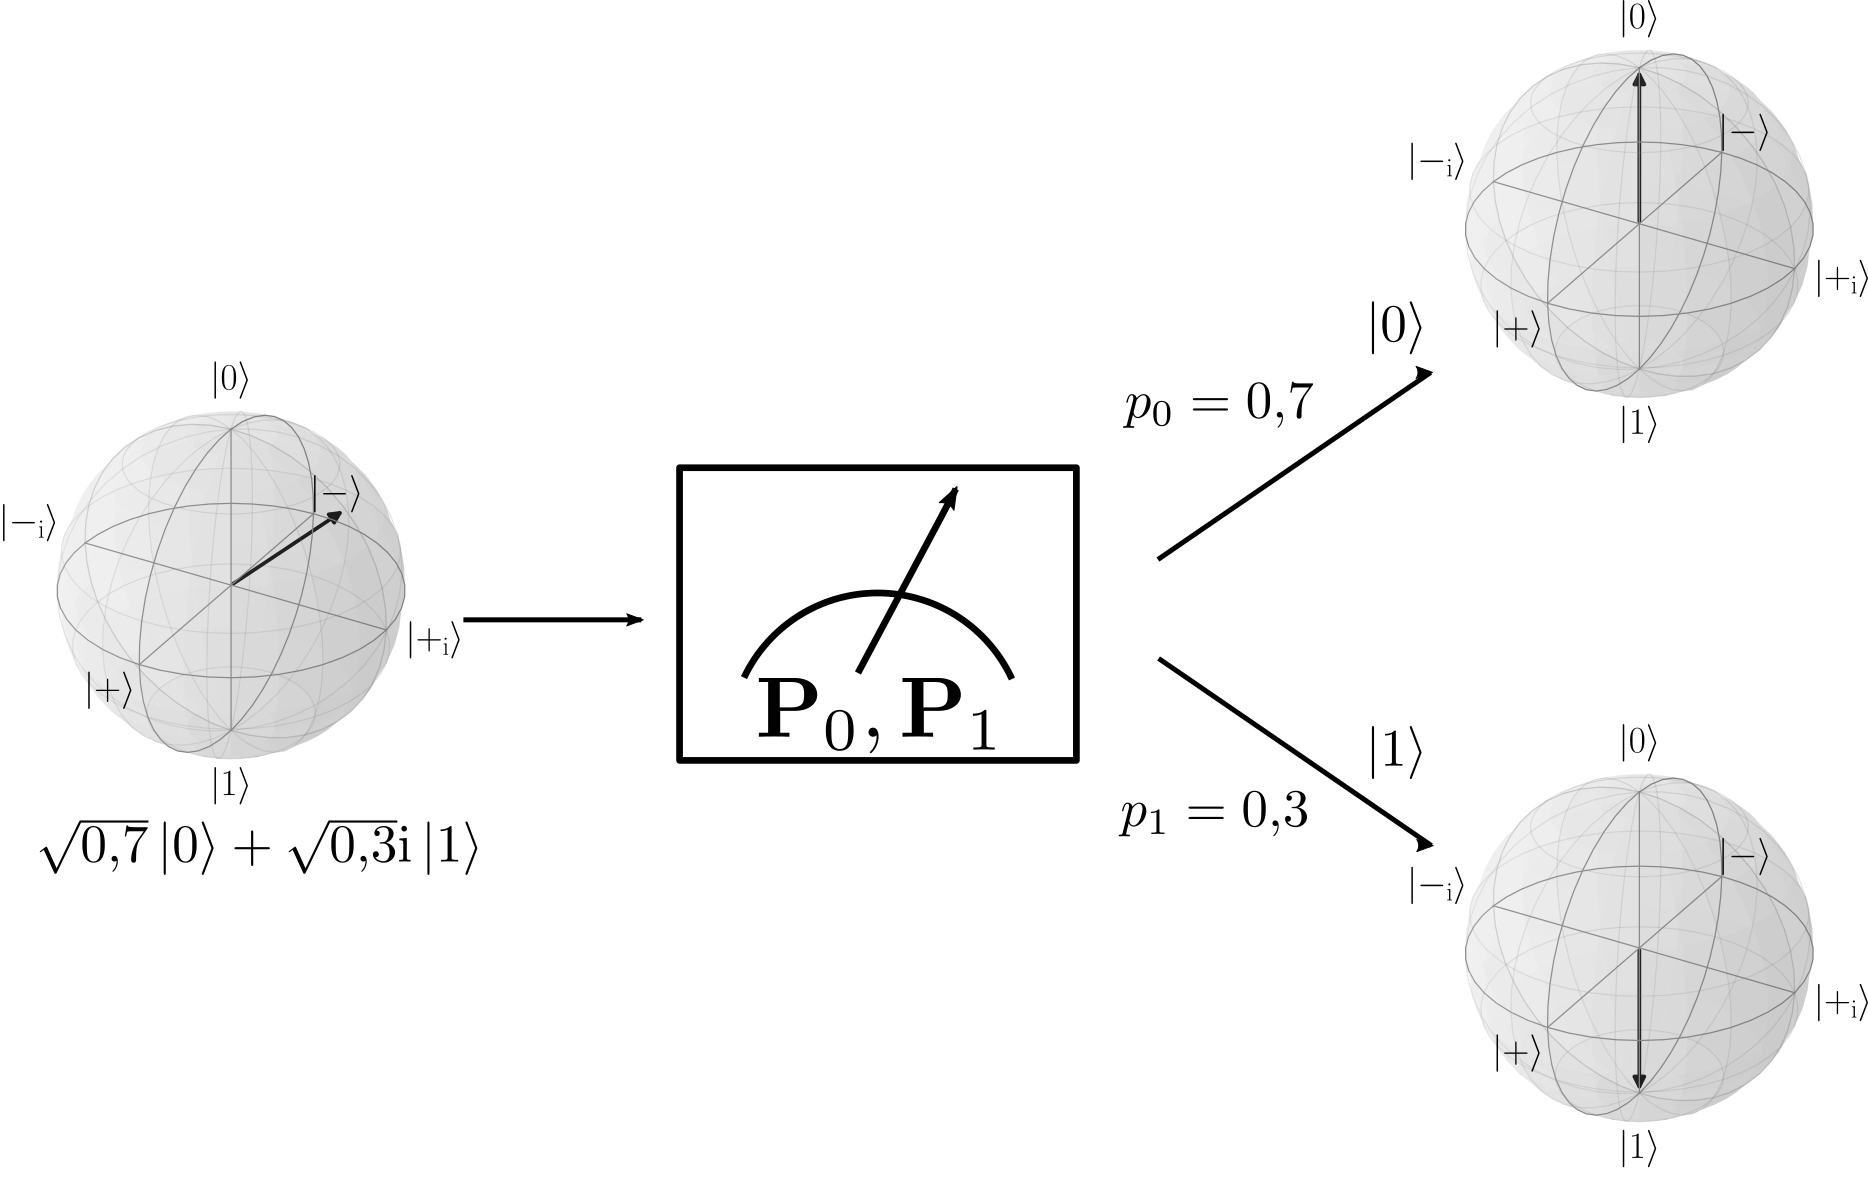
\includegraphics[scale=0.2]{pics/pomiar_sz}
            \end{figure}
        \end{frame}
        %%%%%%%%%%%%%%%%%%%%%%%%%%%%%%%%%%%%%%%%%%%%%%%%%%%%%%%%%%%%%%%%%%%%%%%%%%%%%%%%
        \begin{frame}{Example~$2$ --- part~I}
            \small
            \begin{block}{We will measure the state}
                $$\ket\psi = \sqrt{0.7} \ket{0} + \sqrt{0.3} \mathrm{i}\ket{1} $$
            \end{block}
            \begin{block}{by a measurement}
                %\vspace{0.3cm}
                \begin{equation*}
                    A = \{-_\mathrm{i}, +_\mathrm{i}\}, \quad  Q = \left\{Q_{-_\mathrm{i}}  = 
                    \frac{1}{2}
                    \begin{bmatrix}
                        1 & \mathrm{i}\\
                        -\mathrm{i} & 1
                    \end{bmatrix}, \  
                    Q_{+_\mathrm{i}} =  \frac{1}{2}
                    \begin{bmatrix}
                        1 & -\mathrm{i}\\
                        \mathrm{i} & 1
                    \end{bmatrix}\right\}.
                \end{equation*}
            \end{block}
            \begin{block}{Probabilities of obtaining outcomes $-_\mathrm{i}$ and 
                $+_\mathrm{i}$}
                %\vspace{-0.5cm}
                \begin{equation*}
                    \begin{split}
                        p(-_\mathrm{i}) &= \bra{\psi} Q_{-_\mathrm{i}} \ket{\psi} = 
                        \begin{bmatrix}
                            \sqrt{0.7} & -\sqrt{0.3}\mathrm{i}
                        \end{bmatrix}
                        \frac{1}{2}
                        \begin{bmatrix}
                            1 & \mathrm{i}\\
                            -\mathrm{i} & 1
                        \end{bmatrix}
                        \begin{bmatrix}
                            \sqrt{0.7} \\
                            \sqrt{0.3}\mathrm{i}
                        \end{bmatrix}
                        = \frac{1}{10} (5-\sqrt{21})
                        \approx 0.042,  \\
                        % % % % % % % % % % % % % % % % % % % % % % % % % % % %5
                        p(+_\mathrm{i}) &= \bra{\psi} Q_{+_\mathrm{i}} \ket{\psi} = 
                        \begin{bmatrix}
                            \sqrt{0.7} & -\sqrt{0.3}\mathrm{i}
                        \end{bmatrix}
                        \frac{1}{2}
                        \begin{bmatrix}
                            1 & -\mathrm{i}\\
                            \mathrm{i} & 1
                        \end{bmatrix}
                        \begin{bmatrix}
                            \sqrt{0.7} \\
                            \sqrt{0.3}\mathrm{i}
                        \end{bmatrix}
                        = \frac{1}{10} (5+\sqrt{21})
                        \approx 0.958.
                    \end{split}
                \end{equation*}
            \end{block}
        \end{frame}
        %%%%%%%%%%%%%%%%%%%%%%%%%%%%%%%%%%%%%%%%%%%%%%%%%%%%%%%%%%%%%%%%%%%%%%%%%%%%%%%%
        \begin{frame}{Example~$2$ --- part~II}
            \begin{block}{Conditional states after the measurement}
                \begin{equation*}
                    \begin{split}
                        \ket{\psi}_{-_\mathrm{i}} &= 
                        \frac{Q_{-_\mathrm{i}}\ket{\psi}}{\sqrt{\bra{\psi}Q_{-_\mathrm{i}}\ket{\psi}}}
                        = \frac{1}{\sqrt{\frac{1}{10} (5-\sqrt{21})}}
                        \frac{1}{2}
                        \begin{bmatrix}
                            1 & \mathrm{i}\\
                            -\mathrm{i} & 1
                        \end{bmatrix}
                        \begin{bmatrix}
                            \sqrt{0.7} \\
                            \sqrt{0.3}
                        \end{bmatrix}
                        = \frac{1}{\sqrt{2}}
                        \begin{bmatrix}
                            1 \\
                            - \mathrm{i}
                        \end{bmatrix}
                        = \ket{-_{\mathrm{i}}}\\
                        %%%%%%%%%%%%%%%%%%
                        \ket{\psi}_{+_\mathrm{i}} &= 
                        \frac{Q_{+_\mathrm{i}}\ket{\psi}}{\sqrt{\bra{\psi}Q_{+_\mathrm{i}}\ket{\psi}}}
                        = \frac{1}{\sqrt{\frac{1}{10} (5+\sqrt{21})}}
                        \frac{1}{2}
                        \begin{bmatrix}
                            1 & - \mathrm{i}\\
                            \mathrm{i} & 1
                        \end{bmatrix}
                        \begin{bmatrix}
                            \sqrt{0.7} \\
                            \sqrt{0.3}
                        \end{bmatrix}
                        = \frac{1}{\sqrt{2}}
                        \begin{bmatrix}
                            1 \\
                            \mathrm{i} 
                        \end{bmatrix}
                        =\ket{+_{\mathrm{i}}}
                    \end{split}
                \end{equation*}
            \end{block}
        \end{frame}
        %%%%%%%%%%%%%%%%%%%%%%%%%%%%%%%%%%%%%%%%%%%%%%%%%%%%%%%%%%%%%%%%%%%%%%%%%%%%%%%%
        \begin{frame}{Example~$2$ --- part~III}
            \begin{figure}
                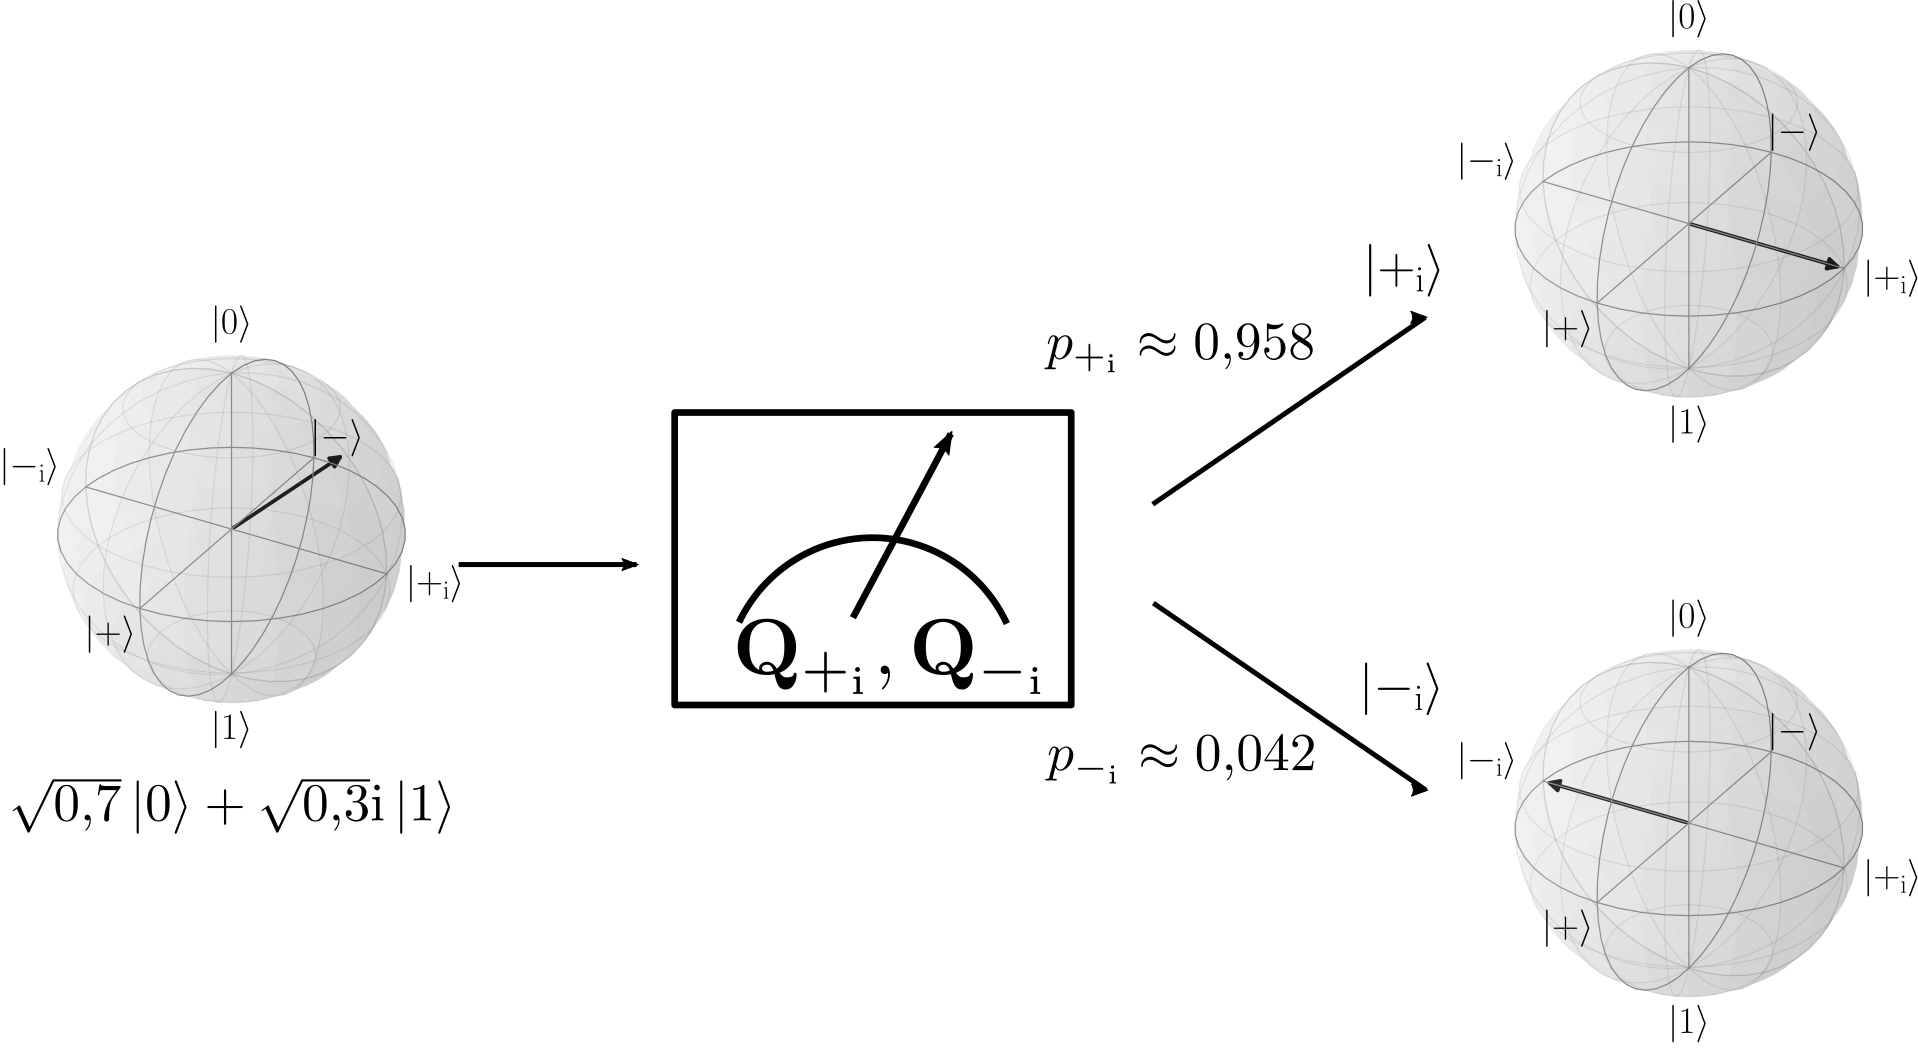
\includegraphics[scale=0.2]{pics/pomiar_sy}
            \end{figure}
        \end{frame}
        %%%%%%%%%%%%%%%%%%%%%%%%%%%%%%%%%%%%%%%%%%%%%%%%%%%%%%%%%%%%%%%%%%%%%%%%%%%%%%%%
        \subsection{Quantum channels}
        %%%%%%%%%%%%%%%%%%%%%%%%%%%%%%%%%%%%%%%%%%%%%%%%%%%%%%%%%%%%%%%%%%%%%%%%%%%%%%%%
        \begin{frame}{Quantum evolution}
            \begin{center}
                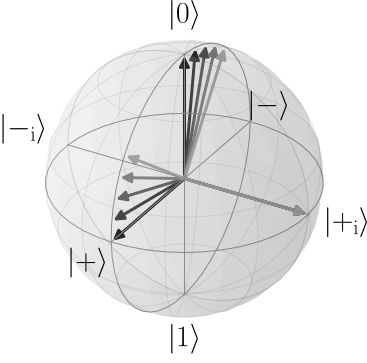
\includegraphics[width=0.4\textwidth]{pics/Ry}\\
                Rotation around y-axis
            \end{center}
        \end{frame}
        %%%%%%%%%%%%%%%%%%%%%%%%%%%%%%%%%%%%%%%%%%%%%%%%%%%%%%%%%%%%%%%%%%%%%%%%%%%%%%%%
        \begin{frame}{Quantum evolution}
            \begin{center}
                \includegraphics[width=0.4\textwidth]{pics/Rz}\\
                Rotation around z-axis
            \end{center}
        \end{frame}
        %%%%%%%%%%%%%%%%%%%%%%%%%%%%%%%%%%%%%%%%%%%%%%%%%%%%%%%%%%%%%%%%%%%%%%%%%%%%%%%%
        \subsection{Entanglement and Bell states}
        %%%%%%%%%%%%%%%%%%%%%%%%%%%%%%%%%%%%%%%%%%%%%%%%%%%%%%%%%%%%%%%%%%%%%%%%%%%%%%%%
        \begin{frame}{Composition of quantum systems}
            \textbf{Tensor product} for \textbf{two qubit} states 
            \begin{equation}\nonumber
                \ket{\psi}=\begin{bmatrix}
                    \alpha\\
                    \beta
                \end{bmatrix}=\alpha\ket{0}+\beta\ket{1},
            \end{equation}
            \begin{equation*}
                \ket{\phi}=\begin{bmatrix}
                    \gamma\\
                    \delta
                \end{bmatrix}=\gamma\ket{0}+\delta\ket{1},
            \end{equation*}
            and their joint state in $\mathbb{C}^2\otimes\mathbb{C}^2$ 
            \begin{equation*}
                \begin{split}
                    \ket{\psi}\otimes\ket{\phi}=
                    \begin{bmatrix}
                        \alpha \gamma\\
                        \alpha \delta\\
                        \beta \gamma\\
                        \beta \delta
                    \end{bmatrix},
                \end{split}
            \end{equation*}
            \begin{equation*}
                \begin{split}
                    \ket{\psi}\otimes\ket{\phi} =
                    & \alpha \gamma \ket{0}\otimes\ket{0}  
                    + \alpha \delta \ket{0}\otimes\ket{1} 
                    + \beta \gamma \ket{1}\otimes\ket{0}  
                    + \beta \delta \ket{1}\otimes\ket{1},
                \end{split}
            \end{equation*}
            \begin{equation*}
                \begin{split}
                    \ket{\psi\phi}=
                    & \alpha \gamma \ket{00}  
                    + \alpha \delta \ket{01} 
                    + \beta \gamma \ket{10}  
                    + \beta \delta \ket{11}.
                \end{split}
            \end{equation*}
        \end{frame}
        %%%%%%%%%%%%%%%%%%%%%%%%%%%%%%%%%%%%%%%%%%%%%%%%%%%%%%%%%%%%%%%%%%%%%%%%%%%%%%%%
        \begin{frame}{Entanglement}
            Recall the product state
            \begin{equation*}
                \begin{split}
                    \ket{\psi\phi}
                    &= \alpha \gamma \ket{00}  
                    + \alpha \delta \ket{01} 
                    + \beta \gamma \ket{10}  
                    + \beta \delta \ket{11},
                \end{split}
            \end{equation*}
            and consider another state
            \begin{equation*}
                \ket{\Psi}
                = a \ket{00}  
                + b \ket{01} 
                + c \ket{10}  
                + d \ket{11}.
            \end{equation*}
            \vspace{-0.5cm}
            \begin{block}{Question}
                Can we always find coefficients which satisfy 
                \begin{equation*}
                    \begin{split}
                        a&= \alpha \gamma  \\
                        b&=  \alpha \delta  \\
                        c&= \beta \gamma   \\
                        d&=  \beta \delta ? 
                    \end{split}
                \end{equation*}
            \end{block}
        \end{frame}
        %%%%%%%%%%%%%%%%%%%%%%%%%%%%%%%%%%%%%%%%%%%%%%%%%%%%%%%%%%%%%%%%%%%%%%%%%%%%%%%%
        \begin{frame}{Entanglement}
            \begin{center}
                %    $\frac{1}{\sqrt{2}}\left(\qk{z1}\qk{z1}+\qk{z2}\qk{z2}\right)$\\
                \begin{block}{Bell State}
                    \begin{equation*}
                        \begin{split}
                            \ket{\Phi^+}=
                            \frac{1}{\sqrt{2}}{\left(\ket{00}+
                            \ket{11}\right)}.
                        \end{split}
                    \end{equation*}
                    \begin{equation*}
                        \ket{\Phi^+} \stackrel{?}{=}
                        \alpha \gamma \ket{00}  
                        + \alpha \delta \ket{01} 
                        + \beta \gamma \ket{10}  
                        + \beta \delta \ket{11},
                        %\psi_0\phi_0\ket{0}\otimes\ket{0}+
                        %\psi_0\phi_1\ket{0}\otimes\ket{1}+
                        %\psi_1\phi_0\ket{1}\otimes\ket{0}+
                        %\psi_1\phi_1\ket{1}\otimes\ket{1}
                    \end{equation*}
                \end{block}
                %%%%%%%%%%%%%%%%%%%%%%%%%%%%%%%%%%%%%%%%%%%%%%%%%%%%%%%%%%%%%%%%%%%%%%%%%%%%%%%%
                \begin{block}{Contradiction}
                    \begin{equation*}
                        \begin{split}
                            \alpha \gamma  & = \beta \delta = \frac{1}{\sqrt{2}},\\
                            \alpha \delta & = \beta \gamma = 0.
                        \end{split}
                    \end{equation*}
                \end{block}
            \end{center}
        \end{frame}